%Empieza configuracion de capitulo
\setstretch{1.0}
\titleformat{\chapter}[block]{\Large\bfseries}{CAP'ITULO \Huge\thechapter\vspace{25 pt}}{0 pt}{\\\fontsize{26}{36}\selectfont}
\titlespacing{\chapter}{0 pt}{30 pt}{50 pt}[0 pt]
\titleformat{\section}{\Large\bfseries}{\thesection}{0 pt}{\hspace{30 pt}}
\titleformat{\subsection}{\large\bfseries}{\thesubsection}{0 pt}{\hspace{30 pt}}
\pagestyle{fancy}
\fancyhead[LO,LE]{\footnotesize\emph{\leftmark}}
\fancyhead[RO,RE]{\thepage}
\fancyfoot[CO,CE]{}
\newcommand{\tabitem}{~~\llap{\textbullet}~~}
%Termina configuracion de capitulo

\chapter{Descripci'on del sistema} %Cambia al nombre de tu capitulo
\setstretch{1.5} %Regresa el interlineado a 1.5

\normalsize
\noindent
En el presente cap'itulo se describir'an los formatos de los archivos descargados, como tambi'en el proceso de obtenci'on de datos, la arquitectura implementada, algunos benchmarketings de software de post-procesamiento, y la explicaci'on del meta-modelo de los datos.\\

Se muestra el funcionamiento del proceso de descarga, el dise'no y desarrollo de la aplicaci'on que extrae y carga los datos hacia el meta-modelo.

\section{Obtenci'on de datos}
\noindent
El primer paso y m'as importante para el desarrollo del proyecto fue la consecuci'on de los datos, ya que en base a ellos se implementa la soluci'on propuesta. Para este proceso se realiz'o un \emph{benchmarketing} de los principales proveedores de datos a nivel mundial. Una vez hecho esto se seleccion'o el que nos pod'ia dar mayores accesos en tiempo real.\\

A continuaci'on, se muestra una tabla con el resultado del \emph{benchmarketing}.\\

\begin{table}[H]
\begin{center}
\scalebox{0.75}{	
\begin{tabular}[0.4\textwidth]{@{\extracolsep{\fill}} | l || c | l | l | l |}
\hline
\textbf{Organizaci'on} & \textbf{Tiempo real} & \textbf{Software o FTP}	& \textbf{\emph{Open data}} & \textbf{\emph{URL}}	\\ \hline \hline
UNAVCO/UNIDATA	&	Si	& Local Data Manager & Si & www.unidata.ucar.edu\\ \hline
CDDIS &	No & Servicio FTP & Si & cddis.nasa.gov\\ \hline
IGS	& No & Servicio FTP & Si & www.igs.org\\ \hline
IGS & Si & BNC NTrip Client & Si & www.igs.org\\ \hline
Jet Propulsion Laboratory & Si & GIPSY & No & gipsy-oasis.jpl.nasa.gov\\ \hline
EUREF Permanent Network	& No & Servicio FTP & Si & www.epncb.oma.be\\ \hline
EUREF Permanent Network & Si & BNC NTrip Client & Si & www.epncb.oma.be\\ \hline
Continuously Operating Reference Station & No & Servicio FTP & Si & www.ngs.noaa.gov/CORS/\\ \hline
Ordnance Survey & No & Servicio FTP & Si & www.ordnancesurvey.co.uk\\ \hline
British Isles continuous GNSS Facility & No & Servicio FTP & Si & www.bigf.ac.uk\\ \hline
Royal Observatory of Belgium & Si & BNC NTrip Client & Si & gnss.be\\ \hline
Royal Observatory of Belgium & No & Servicio FTP & Si & gnss.be\\ \hline
\end{tabular}}
\end{center}
\caption{\emph{Benchmarketing}: proveedores de datos satelitales.}
\end{table}

El proveedor de datos seleccionado fue el IGS \emph{ International GNSS Service} con su servicio de datos en tiempo real a trav'es del protocolo NTRIP usando el cliente \emph{BNC Ntrip Client} proporcionado por esta misma organizaci'on. Se escogi'o este proveedor porque que cuenta con muchas oraganizaciones aliadas y afiliadas para su servicio de transmisi'on de datos en tiempo real, adem'as de que proporciona un cliente de software que es de libre uso. De igual manera es la organizaci'on que m'as agrupa usuarios y servicios de datos de los GNSS y de alguna manera es la m'as conocida en ese medio.\\

Se realiz'o el registro a trav'es del sitio web del IGS, solicitando un n'umero grande \emph{streams}, alrededor de 1000, con el objetivo de descargar desde diferentes \emph{broadcasters} afiliados a esta organizaci'on la mayor cantidad de datos en el menor tiempo posible. La respuesta v'ia email por parte de los administradores tard'o aproximadamente una semana, en donde se decia que el registro fue exitoso y que en los pr'oximos d'ias enviar'ian los datos de autentificaci'on. Al pasar varias semanas no se obtuvo respuesta alguna, por lo que se les escribi'o nuevamente tanto por parte del investigador como del asesor de la tesis.\\

Al pasar casi un mes y a'un sin recibir notificaci'on alguna por parte de la organizaci'on, se decidi'o con el asesor, solicitar el registro para el proyecto \emph{Multi-GNSS Experiment (MGEX)}, el cual tiene por objetivo rastrear, cotejar y analizar todas las se'nales GNSS disponibles. Este proyecto nos proporcion'o los accesos necesarios para la descarga de los datos. La 'unica restricci'on de este proyecto es que se otorga el acceso a m'aximo 15 \emph{streams}, de los cuales 5 \emph{streams} pertenecen a la red del IGS, 5 a la red del proyecto MGEX y los 'ultimos 5 a la red \emph{EUREF Permanent Network}. El otorgamiento de los accesos tard'o un d'ia. \\

Despu'es de realizar varias pruebas con los accesos otorgados, se definieron de manera aleatoria los 15 \emph{broadcasters} pertenecientes a la red. \\

En las siguientes tablas se muestran los mapeos realizados de las diferentes estaciones por cada una de las agencias pertenecientes de las cuales se descargaron los datos:\\

\textbf{Caster Host:} mgex.igs-ip.net
\textbf{Caster Port:} 2101
\textbf{Network:} IGS

\begin{table}[H]
\begin{center}
\scalebox{0.72}{	
\begin{tabular}[0.4\textwidth]{@{\extracolsep{\fill}} | l || c | l | l | l | l | l |}
\hline
\textbf{Mounpoint (ID)} & \textbf{Ciudad} & \textbf{Pa'is}	& \textbf{Formato} & \textbf{Sistema} & \textbf{Agencia}	& \textbf{\emph{Bitrate}}\\ \hline \hline
AREG7	&	Arequipa	& Peru & RTCM 3.2 & GPS + GLO & Jet Propulsion Laboratory & 2400\\
& & & & GAL + BDS & &\\
& & & & SBAS & &\\ \hline
CONX7	&	Concepci'on	& Chile & RTCM 3.2 & GPS + GLO & No publicado & 9600\\ 
& & & & GAL + SBAS & &\\ \hline
LPGS7	&	La Plata	& Argentina & RTCM 3.2 & GPS + GLO & Helmholtz-Zentrum Potsdam & 3000\\ 
& & & & GAL & Deutsches GeoForschungsZentrum &\\ \hline
RIO27	&	Rio Grande Do Sul	& Brasil & RTCM 3.2 & GPS + GLO & No publicado & 3000\\ 
& & & & GAL & &\\ \hline
SCRZ7	&	Santa Cruz	& Bolivia & RTCM 3.2 & GPS + GLO & No publicado & 2200\\ 
& & & & GAL & &\\ \hline
\end{tabular}}
\end{center}
\caption{\emph{Broadcasters} pertenecientes a la red del proyecto \emph{MGEX}.}
\end{table}

\textbf{Caster Host: }www.euref-ip.net
\textbf{Caster Port:} 80
\textbf{Network: }EUREF

\begin{table}[H]
\begin{center}
\scalebox{0.72}{	
\begin{tabular}[0.4\textwidth]{@{\extracolsep{\fill}} | l || c | l | l | l | l | l |}
\hline
\textbf{Mounpoint (ID)} & \textbf{Ciudad} & \textbf{Pa'is}	& \textbf{Formato} & \textbf{Sistema} & \textbf{Agencia}	& \textbf{\emph{Bitrate}}\\ \hline \hline
AJAC0	&	Ajaccio	& Francia & RTCM 3.1 & GPS + GLO & Institut National & 4000\\
& & & & & de l`Information Geographique et Forestiere &\\ \hline
ALAC0	&	Alicante	& Espa'na & RTCM 3.0 & GPS + GLO & No publicado & 5000\\ \hline
BOGI0	&	Borowa Gora	& Polonia & RTCM 3.0 & GPS + GLO & Institute of Geodesy and Cartography & 4000\\ \hline
VIS00	&	Visby & Suecia & RTCM 3.0 & GPS + GLO & Lantmateriet, the Swedish mapping, & 6000\\ 
& & & & & cadastral and land registration authority &\\ \hline
ZOUF0	& Cercivento & Italia & RTCM 2.3 & GPS + GLO & Centro Ricerche Sismologiche & 5500\\ \hline
\end{tabular}}
\end{center}
\caption{\emph{Broadcasters} pertenecientes a la red \emph{EUREF}.}
\end{table}

\textbf{Caster Host:} www.igs-ip.net
\textbf{Caster Port:} 2101
\textbf{Network}: IGS

\begin{table}[H]
\begin{center}
\scalebox{0.72}{	
\begin{tabular}[0.4\textwidth]{@{\extracolsep{\fill}} | l || c | l | l | l | l | l |}
\hline
\textbf{Mounpoint (ID)} & \textbf{Ciudad} & \textbf{Pa'is}	& \textbf{Formato} & \textbf{Sistema} & \textbf{Agencia}	& \textbf{\emph{Bitrate}}\\ \hline \hline
ADH10	&	Abu Dhabi	& Emiratos Arabes & RTCM 3.0 & GPS + GLO & No publicado & 9600\\ 
& & Unidos & & & &\\ \hline
ALIC0	&	Alice Springs	& Australia & RTCM 3.1 & GPS + GLO & Geoscience Australia & 1600\\ \hline
BRAZ0	&	Brasilia	& Brasil & RTCM 3.0 & GPS + GLO & Brazilian Institute of Geography & 5000\\
& & & & & and Statistics &\\ \hline
CNMR0	&	Saipan & Estados Unidos & RTCM 3.0 & GPS + GLO & NOAA-National Geodetic Survey & 2000\\ \hline
FFMJ1	& Frankfurt & Alemania & RTCM 3.1 & GPS + GLO &Bundesamt fuer Kartographie und  & 2400\\
& & & & & Geodaesie Department of Geodaesie &\\ \hline
\end{tabular}}
\end{center}
\caption{\emph{Broadcasters} pertenecientes a la red \emph{IGS}.}
\end{table}

\section{Formatos}
\noindent
En esta secci'on se describen en detalle los formatos utilizados por los archivos y se explica el funcionamiento del protocolo de comunicaci'on NTRIP para el intercambio de datos procedentes de los sistemas de posicionamiento global.

\subsection{Raw Data}
\noindent
Los datos primarios (tambi'en conocidos como datos en bruto) es un t'ermino para los datos recogidos a partir de una fuente o \emph{source}. Los datos primarios no han sido objeto de procesamiento o cualquier otra manipulaci'on. \\

Los datos primarios generalmente son las entradas o \emph{inputs} para un programa inform'atico. Estos datos pueden tener los siguientes atributos: posiblemente contienen errores, no est'an validados; est'an en diferentes formatos; no est'an codificados o est'an sin formato.\\

Aunque los datos en bruto tienen el potencial de convertirse en ``informaci'on'', la extracci'on y la organizaci'on, en la mayor'ia de ocasiones requiere del an'alisis y del formato correcto para la presentaci'on de estos.

\subsection{Formato RTCM}
\noindent
La Comisi'on T'ecnica de Radio para Servicios Mar'itimos (\emph{Radio Technical Commission for Maritime Services, RTCM}) es una organizaci'on internacional de normalizaci'on o estandarizaci'on. Es una agencia cient'ifica, profesional y educativa no lucrativa.
Los miembros pertenecientes al RTCM no son individuos particulares sino agencias gubernamentales y no gubernamentales.\\

En los Estados Unidos, la Comisi'on Federal de Comunicaciones (\emph{Federal Communications Commission}) y la Guardia Costera de EE.UU. utilizan est'andares RTCM para especificar sistemas de radar, y sistemas diferenciales de GPS, entre otros.\\

Los mensajes consisten en una secuencia de palabras con 30-bits cada uno. Los 'ultimos seis bits de cada palabra son bits de paridad. Cada mensaje comienza con una cabecera que es de dos o tres palabras de largo. La primera palabra contiene un pre'ambulo fijo, el identificador de tipo de mensaje, y el identificador de la estaci'on de referencia. La segunda palabra contiene la etiqueta del sistema de tiempo, el n'umero de secuencia, la longitud del mensaje, y un indicador de la salud de las estaciones de referencia. En algunos mensajes hay una tercera palabra que se agrega al encabezado. El mensaje total tiene una longitud m'axima de 33 palabras.\\

Los DGPS (\emph{Differential Global Positioning System}) convecionales requieren de los tipos de mensajes 1, 2 y 9 para proporcionar la precisi'on del medidor. La operaci'on RTK (\emph{Real Time Kinematics}) se basa en los tipos de mensajes del rango entre 18 a 21 para proporcionar una precisi'on centim'etrica. Varios sistemas utilizan el formato de mensaje RTCM para transmitir informaci'on confidencial. Por ejemplo, el tipo de mensaje 59, en particular, se puede utilizar como un canal de comunicaci'on para transmitir mensajes cortos.
Los mensajes relacionados con GLONASS est'an disponibles desde la versi'on 2.2. En la tabla 4.5 se ilustran los tipos de mensaje para la versi'on 2.3.\\

RTCM en su versi'on 3, se ha definido para aumentar la eficiencia de la transmisi'on de la informaci'on y para aumentar la integridad de la operaci'on de paridad. La versi'on 3 ha sido especialmente dise'nada para las operaciones de RTK, donde un gran vol'umen de datos se han de transmitir. El mensaje consta de un pre'ambulo de 8 bits, la longitud del mensaje identificador de 10 bits, y 6 bits adicionales en la cabecera reservados para un uso futuro. El campo de datos tiene una longitud m'axima de 1024 bytes seguida de una comprobaci'on de redundancia c'iclica de 24 bits (\emph{cyclic redundancy check, CRC}).\\

Para la transmisi'on de datos RTCM a trav'es de Internet se realiza por medio del protocolo de Internet NTRIP que ha sido definida por la Agencia Federal Alemana para la Cartograf'ia y Geodesia. NTRIP se basa en el protocolo de transferencia de hipertexto (HTTP). Mientras tanto, el formato NTRIP ha sido asumido oficialmente por el RTCM.\\

\begin{table}[H]
\begin{center}
\scalebox{0.8}{	
\begin{tabular}{| l || c | c | l |}
\hline
\textbf{Nombre del documento} & \textbf{Referencia} & \textbf{Versi'on} & \textbf{Comentarios}\\ \hline \hline
\emph{Recommended Standards for Differential } & 10402.3 & 2.3 & Este est'andar se utiliza en todo el mundo \\ 
\emph{GNSS(Global Navigation Satellite} & & & para GNSS diferenciales, tanto mar'itima \\
\emph{Systems) Service} & & & como terrestre.\\ \hline
\emph{Differential GNSS (Global Navigation} & 10403.1 & 3.1 & Es una alternativa m'as eficiente para la \\ 
\emph{Satellite Systems) Services} & & &  referencia 10402.3 \\ \hline
\emph{Standard for Networked Transport of} & 10410.0 & 1 & Protocolo de nivel de aplicaci'on que\\
\emph{RTCM via Internet Protocol (Ntrip)} & & & soporta la transmisi'on de datos\\ 
& & & de cualquier GNSS a trav'es de Internet.\\ \hline
\emph{Standard for Differential Navstar GPS} & 10401.2 & 2 & Esta norma se ocupa de los requisitos de \\
\emph{Reference Stations and Integrity} & & & rendimiento para el equipo que \\ 
\emph{Monitors (RSIM)} & & & emite correcciones DGNSS.\\ \hline
\end{tabular}}
\end{center}
\caption{Est'andares \emph{RTCM}. }
\end{table}

\begin{table}[H]
\begin{center}
\scalebox{0.9}{	
\begin{tabular}{| c || l | }
\hline
\textbf{Tipo de mensaje} & \textbf{Funci'on} \\ \hline \hline
1 & Correciones para DGPS \\ \hline
2 & Correciones para el diferencial delta de GPS\\ \hline
3 & Par'ametros para las estaciones de referencia de GPS\\ \hline
9 & Conjunto parcial de sat'elites GPS\\ \hline
10 & Correcciones diferenciales para P-Code\\ \hline
11 & Correcciones delta para GPS C/A-code L1,L2 \\ \hline
15 & Mensaje de retraso ionosf'erico\\ \hline
17 & GPS ephemerides\\ \hline
18 & Fase de \emph{carrier} sin corregir para RTK\\ \hline
19 & C'odigo de pseudorangos sin corregir para RTK\\ \hline
20 & Correcciones para la fase de \emph{carrier} para RTK\\ \hline
21 & Correciones de los c'odigos de pseudorangos para la fase de \emph{carrier} para RTK\\ \hline
31 & Correcciones diferenciales para GLONASS\\ \hline
32 & Par'ametros para las estaciones de referencia de GLONASS\\ \hline
59 & Mensaje propietario\\ \hline
\end{tabular}}
\end{center}
\caption{Tipos de mensaje, \emph{RTCM} versi'on 2.3. }
\end{table}

\subsection{Formato RINEX}
\noindent
RINEX o \emph{Receiver Independent Exchange} es un formato de texto estandarizado para recopilar las medidas u observaciones proporcionadas por los GNSS. Adem'as permite el procesado \emph{off-line} por varias aplicaciones de software, independientemente de cual sea el fabricante tanto del receptor como de la aplicaci'on inform'atica.\\

La versi'on m'as com'un en la actualidad es la 2.10, que permite el almacenamiento de medidas de pseudodistancias, fase de portador y Doppler.\\

En las siguientes tablas se describen los campos que contiene el formato RINEX en su versi'on 2.11 para el tipo de archivo \emph{Observation File}, el cual fue utilizado en el desarrollo de la presente investigaci'on:\\

\textbf{Cabecera del archivo o \emph{header}}

\begin{table}[H]
\begin{center}
\scalebox{0.6}{	
\begin{tabular}{| l || l | l | }
\hline
\textbf{Campo} & \textbf{Descripci'on} & \textbf{Ejemplo}\\ \hline \hline
RINEX VERSION / TYPE & \tabitem Versi'on del formato (2.11) &      2.11           Observation data    Mixed \\
& \tabitem Tipo de archivo (`O' for Observation Data)  & \\
& \tabitem Sistema: nulo o `G': GPS  & \\ 
& \tabitem `R': GLONASS & \\
& \tabitem `S': Geostationary signal payload  & \\
& \tabitem `E' : Galileo & \\
& \tabitem `M': Mixed & \\ \hline
PGM / RUN BY / DATE & \tabitem Nombre del programa o aplicaci'on que cre'o el archivo & BNC 2.10            Julio               25-abr.-14 18:09\\
& \tabitem Nombre de la agencia o persona que creo el archivo & \\
& \tabitem Fecha de creaci'on del archivo & \\ \hline
COMMENT & Comentarios adicionales & RTCM 3 www.igs-ip.net/ADH10 \\ \hline
MARKER NAME & Nombre de la antena del orig'en de los datos & ADH10 \\ \hline
OBSERVER / AGENCY & Nombre de la agencia u observador & gAGE                UPC: Technical University of Catalonia \\ \hline
REC \# / TYPE / VERS & N'umero del receptor, tipo y versi'on de software & IR2200716006        ASHTECH UZ-12       CQ00 \\ \hline
ANT \# / TYPE & N'umero y tipo de antena & 482 AOAD/M\_T NONE \\ \hline
APPROX POSITION XYZ & Posici'on aproximada de la antena en las coordenadas X, Y y Z &    4789028.4701    176610.0133   4195017.0310 \\ \hline
ANTENNA: DELTA H/E/N & \tabitem Altura de la superficie inferior de la antena sobre la fuente de origen &          0.9030         0.0000         0.0000 \\
& \tabitem Singularidades del centro de la antena con respecto a la fuente de origen, & \\ 
& al este y al norte (todas las unidades en metros) & \\ \hline
WAVELENGTH FACT L1/2 & \tabitem Factores por defecto de longitud de onda para L1 y L2 (GPS solamente) &      1     1 \\
& 1: ambig\"uedades de ciclo completo & \\
& 2: las ambig\"uedades de ciclo medio (cuadratura) & \\
& 0 (en L2): Frecuencia simple de instrumento & \\
& cero o en blanco & \\
& \tabitem El registro del factor de longitud de onda es opcional para GPS & \\
& y obsoleto para los otros sistemas. Los factores de longitud de onda & \\
& por defecto es 1. Si existe el registro, este debe preceder a alg'un  & \\ 
& registro espec'ifico de sat'elite & \\ \hline
\# / TYPES OF OBSERV & \tabitem N'umero de diferentes tipos de observaciones  &      8    C1    P1    L1    S1    C2    P2    L2    S2 \\
& almacenados en el archivo & \\
& \tabitem Tipos de observaciones & \\
& \tabitem C'odigo de observaci'on & \\
& \tabitem C'odigo de frecuencia & \\
& \tabitem Si hay m'as de 9 tipos de observaciones se & \\
& contin'ua en la siguiente l'inea & \\
& \tabitem Los siguientes tipos de observaciones est'an definidos & \\ \hline
\end{tabular}}
\end{center}
\caption{\emph{Header Observation file}, primera parte, RINEX versi'on 2.11.}
\end{table}

\begin{table}[H]
\begin{center}
\scalebox{0.6}{	
\begin{tabular}{| l || l | l | }
\hline
\textbf{Campo} & \textbf{Descripci'on} & \textbf{Ejemplo}\\ \hline \hline
\# / TYPES OF OBSERV & \tabitem C: Pseudorang & 8    C1    P1    L1    S1    C2    P2    L2    S2 \\ 
& GPS: C/A, L2C & \\
& GLONASS: C/A & \\
& GALILEO: ALL & \\
& P: Pseudorange GPS y GLONASS & \\
& L: Carrier phase & \\
& D: Doppler frequency & \\
& S: Intensidades de se'nal sin procesar o valores SNR dada por el & \\ & receptor de las observaciones de la fase respectivas & \\
& \tabitem C'odigos de frecuencias: & \\
& \tabitem 1 & \\
& GPS: L1 & \\
& GLONASS: G1 & \\
& GALILEO: E2-L1-E1 & \\
& SBAS: L1 & \\
& \tabitem 2 & \\
& GPS: L2 & \\
& GLONASS: G2 & \\
& \tabitem 5 & \\
& GALILEO: E5a & \\
& SBAS: L5 & \\
& \tabitem 6 & \\
& GALILEO: E6 & \\
& \tabitem 7 & \\
& GALILEO: E5b & \\
& \tabitem 8 & \\
& GALILEO: E5a+b & \\
& \tabitem Unidades: & \\
& Phase: Ciclos completos & \\
& Pseudorange: metros & \\
& Doppler: Hz & \\
& SNR: Depende del receptor & \\ \hline
TIME OF FIRST OBS & \tabitem Tiempo del primer registro observable &   2014     4    25    18     9   29.0000000     GPS         \\
& 4 d'igitos para el a'no & \\
& Mes & \\
& D'ia & \\
& Hora & \\
& Minuto & \\
& Segundo & \\
& \tabitem Sistema del tiempo & \\
& GPS: Sistema de tiempo GPS & \\
& GLO: Sistema de tiempo UTC & \\
& GAL: Sistema de tiempo de GALILEO & \\
& Campo obligatorio cuando el archivo es mixto, es decir,& \\
& contiene registros de los sistemas GPS/GLONASS & \\ \hline
END OF HEADER & Fin de la cabecera o \emph{header} del archivo & \\ \hline
\end{tabular}}
\end{center}
\caption{\emph{Header Observation file}, segunda parte, RINEX versi'on 2.11.}
\end{table}

\textbf{Cuerpo o \emph{body} del archivo}

\begin{table}[H]
\begin{center}
\scalebox{0.6}{	
\begin{tabular}{| l || l | l | }
\hline
\textbf{Campo} & \textbf{Descripci'on} & \textbf{Ejemplo}\\ \hline \hline
EPOCH/SAT or EVENT FLAG & \tabitem Epoch o 'epoca &  14 04 25 18 09 29.0000000  0  8R 7R 6R21R11R23R22R13R12 \\
&  2 d'igitos para el a'no & \\
& Mes & \\
& D'ia & \\
& Hora & \\
& Minuto & \\
& Segundo & \\
& \tabitem Epoch flag o bandera de 'epoca & \\
& 0: OK & \\
& 1: Falla el'ectrica entre la 'epoca anterior y la actual & \\
& 3: Nueva ocupaci'on de sitio & \\
& 4: Continua informaci'on de cabecera & \\
& 5: Evento externo & \\ 
& 6: Registros de deslizamiento de ciclo seguidos & \\
& opcionalmente del informe de detectado y reparado & \\
& \tabitem Campo obligatorio cuando el archivo es mixto,& \\
& es decir, contiene registros de los sistemas GPS/GLONASS & \\
& Si hay m'as de 12 sat'elites se continua en la siguiente l'inea & \\ \hline
OBSERVATIONS & \tabitem Valores de las observaciones hechas & 21889866.636 0.000 117178181.112 45.000 0.000\\
& para cada uno de los tipos especificados en la & 21889875.056    91138588.078 41.000 \\
& cabecera o header del archivo. El orden de los valores & \\
& es dado por el orden de los tipos de observaciones & \\ 
& de la cabecera (campo \# / TYPES OF OBSERV) & \\
& \tabitem  El pen'ultimo d'igito de cada valor representa la & \\
& p'erdida del indicador de bloqueo o Loss of lock indicator & \\ 
& (LLI). Solo aplica para los tipos L1 y L2: & \\
& 0 o en blanco: OK o no conocido & \\
& Bit 0 set: Bloqueo perdido entre el anterior y  & \\
& el actual registro de observaci'on: posible & \\ 
& deslizamiento de ciclo & \\
& Bit 1 set: Factor de longitud de onda opuesta a & \\
& la definida para el sat'elite por un HECHO DE ONDA &\\
& (WAVELENGTH FACT) anterior, L1 / 2 o contraria & \\
& a los valores predeterminados. V'alido s'olo para & \\
& la 'epoca actual & \\
& Bit 2 set: Valor bajo Antispoofing & \\
& \tabitem El 'ultimo d'igito de cada valor representa & \\
& la intensidad de la se'nal para ese tipo de observable: & \\
& 1: Intensidad m'inima posible & \\
& 5: Umbral de tasa buena S/N & \\
& 9: Intensidad de se'nal m'axima & \\
& 0 o en blanco: no conocido & \\ \hline
\end{tabular}}
\end{center}
\caption{\emph{Body Observation file}, RINEX versi'on 2.11.}
\end{table}

\subsection{Protocolo NTRIP}
\noindent
Ntrip fue desarrollado por la Agencia Alemana Federal de Cartograf'ia y Geodesia (BKG) y el Departamento de Ciencias de la Computaci'on de la Universidad de Dortmund. Ntrip fue lanzado en septiembre de 2004 como ``\emph{RTCM Recommended Standards for Networked Transport of RTCM via Internet Protocol (Ntrip), Version 1.0}''. La versi'on actual del protocolo es la Versi'on 2.0 bajo la enmienda 1 del 28 de junio de 2011. \\

\emph{Networked Transport of RTCM via Internet Protocol} NTRIP es un protocolo para la transmisi'on de GPS diferencial (DGPS) de datos a trav'es de Internet, de acuerdo con las especificaciones publicadas por la RTCM. Ntrip es un protocolo gen'erico, sin estado, basado en el protocolo de transferencia de hipertexto HTTP/1.1 y el cual se ha mejorado para los flujos de datos (\emph{data streams}) de los GNSS.\\

NTRIP ha sido dise'nado para la difusi'on de los datos de correcci'on diferencial u otros tipos de \emph{streaming} de datos GNSS a usuarios fijos o m'oviles a trav'es de Internet, lo que permite conexiones simult'aneas de computadores, port'atiles o PDA's. Ntrip es compatible con el acceso inal'ambrico (WI-FI) a Internet por medio de redes de IP m'ovil como GSM, GPRS, EDGE, UMTS.\\

NTRIP se implementa en tres componentes de software del sistema: NTRIPClients, NTRIPServers y NTRIPCasters. El NTRIPCaster es el programa servidor HTTP real mientras que NtripClient y NTRIPServer est'an actuando como clientes HTTP.\\

NTRIP es un protocolo est'andar abierto. El protocolo se puede descargar libremente desde BKG y hay una implementaci'on de c'odigo abierto disponible desde \emph{software.rtcm-ntrip.org}.

\subsubsection{Arquitectura del protocolo NTRIP}
\noindent
El protocolo se compone de los siguientes elementos:
\begin{enumerate}
\item \emph{NtripSources}, que generan flujos de datos en una ubicaci'on espec'ifica, 
\item \emph{NTRIPServers}, que transfieren los flujos de datos de una fuente al \emph{NTRIPCaster},
\item \emph{NTRIPCaster}, es el componente principal del sistema, y 
\item \emph{NTRIPClients}, que finalmente acceden a los flujos de datos de \emph{NtripSources} deseados en el \emph{NTRIPCaster}.
\end{enumerate}

En la siguiente figura se ilustra la arquitectura de componenetes del protocolo:

\begin{figure}[H]
\centering
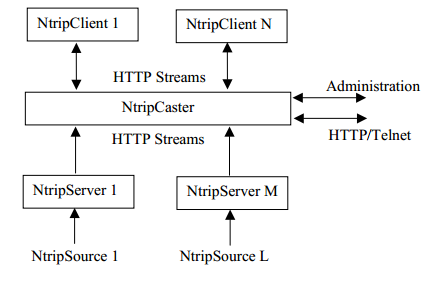
\includegraphics[width=0.95\textwidth]{images/Ntrip_Arquitectura}
\caption{Arquitectura protocolo NTRIP.}
\label{fig:4.1}
\end{figure}

\subsection{Nomenclatura archivos RINEX}
\noindent
El software BNC sigue las conveciones del formato RINEX en su versi'on 2.0. Este software a'un no soporta los nombres extendidos que vienen en la versi'on 3.02. \\

Los nombres de los archivos son derivados por el software para los 4 primeros caracteres de la clave o identificaci'on del \emph{mounpoint}. Por ejemplo para el \emph{mounpoint} ALAC0 de la ciudad de Alicante, Espa'na, el nombre de su \emph{observation file} ser'ia:\\

ALAC(ddd)(h).(yy)O,\\

donde (ddd) es el d'ia del a'no, la (h) es una letra la cual corresponde a una hora larga en el formato de tiempo UTC; y (yy) son los 'ultimos dos d'igitos del a'no.\\

Sin embargo, si existe m'as de un \emph{stream} con la misma identificaci'on de \emph{mounpoint}, la cadena de identificaci'on se divide en dos partes o dos subcadenas y ambas partes conforman el nombre del archivo, como se muestra a continuaci'on:\\

AL(ddd)(h)\_AC.(yy)O.\\

Los nombres de los archivos para todos los intervalos menor a una hora, tienen la convenci'on para los \emph{observation files} de 15 minutos, como sigue:\\

ALAC(ddd)(h)(mm).(yy)O,\\

donde (mm) es el minuto de inicio dentro de la hora.\\

\section{Arquitectura del sistema}
\noindent
En la presente secci'on se describe cada uno de los elementos que componen la arquitectura implementada y la cual se propone como soluci'on. \\

La arquitectura general del sistema de tranferencia y extracci'on del conocimiento para los GNSS (STECG) est'a dividida en 4 grandes capas: componentes externos, comunicaci'on, software y almacenamiento. 

\begin{itemize}
\item Componentes externos: Son todos aquellos elementos que conforman la parte f'isica del sistema, tales como los sat'elites de la constelaci'on GLONASS, las antenas receptoras, las estaciones de control de datos y los \emph{broadcasters}.

\item Comunicaci'on: Es la capa que permite la transmisi'on de flujos de datos o \emph{data streams} a trav'es de la red.

\item Software: Est'a compuesto por todos los elementos de software utilizados y desarrollados para la extracci'on, transformaci'on y almacenamiento de los datos.

\item Almacenamiento: Esta capa se compone del metamodelo l'ogico y la base de datos donde se guarda la informaci'on relevante de los datos descargados.
\end{itemize}

\begin{figure}[H]
\centering
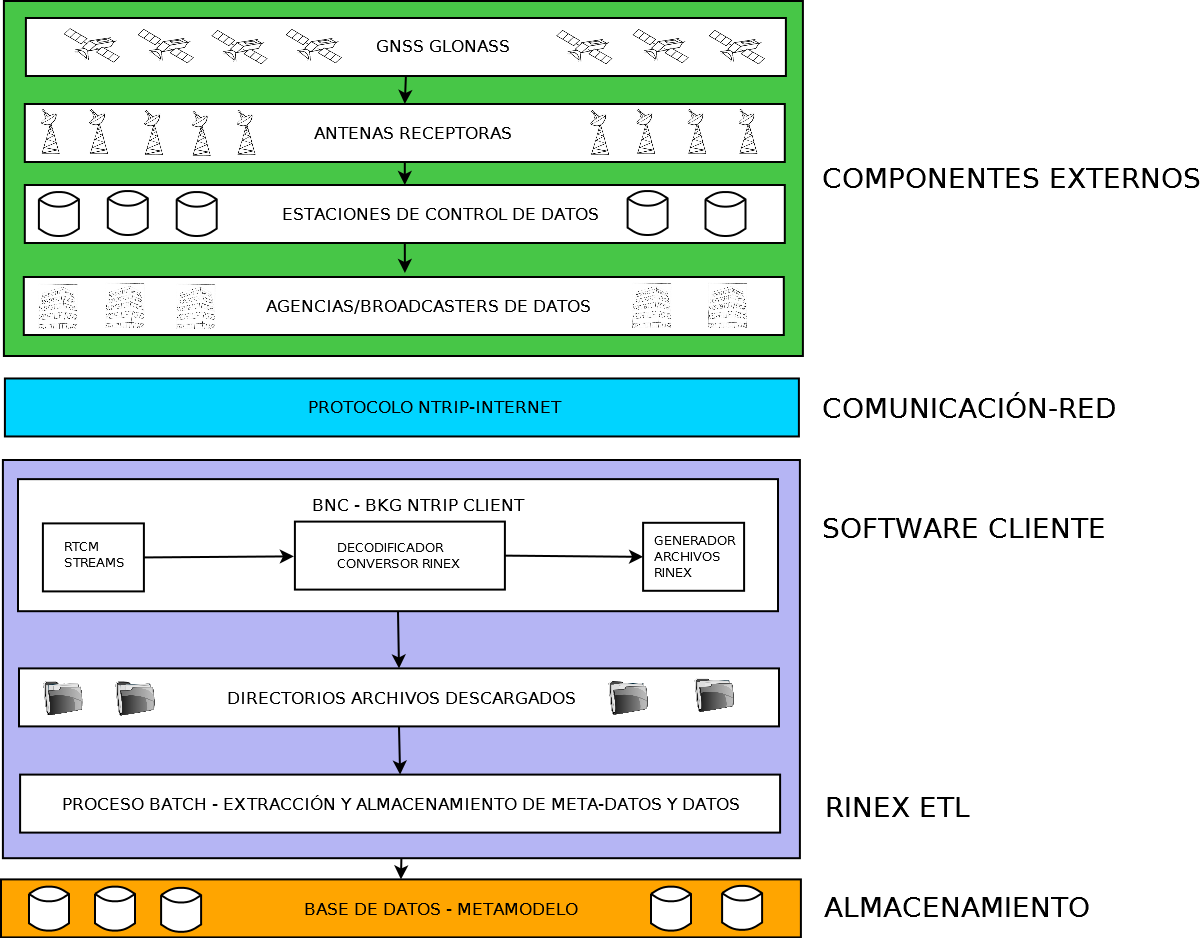
\includegraphics[width=0.95\textwidth]{images/ARQUITECTURA_SISTEMA}
\caption{Arquitectura del sistema}
\label{fig:4.2}
\end{figure}

\subsection{Componentes externos}
\noindent
A continuaci'on, se relacionan todos los elementos que pertenecen a esta capa de la arquitectura.

\begin{enumerate}
\item \textbf{GLONASS:} Es un GNSS que tiene una constelaci'on de 31 sat'elites (24 en activo, 3 sat'elites de repuesto, 2 en mantenimiento, uno en servicio y uno en pruebas) situados en tres planos orbitales con 8 sat'elites cada uno.
Son la fuente principal donde se producen los datos contenidos en los archivos RINEX.
\item \textbf{Antenas receptoras:} Son las antenas que reciben las se'nales con los datos procedentes de GLONASS. Son el intermediario entre la comunicaci'on de GLONASS y las estaciones de control.
\item \textbf{Estaciones de control de datos:} Son las estaciones que se encargan de la operaci'on, control y supervisi'on de los GNSS. All'i se almacenan los datos trasmitidos por GLONASS. Se realiza intercambio de informaci'on con los GNSS en caso de sincronizaci'on de eventos y reconfiguraci'on de alg'un sat'elite.
\item \textbf{Agencias/Broadcasters de datos:} Son aquellas agencias, organizaciones o institutos que recoletan, almacenan, procesan e investigan los datos enviados por los GNSS y a su vez retrasnmiten estos datos por Internet a cualquier interesado en el procesamiento e investigaci'on cient'ifica de esta informaci'on.
Cabe aclarar que la retransmisi'on de los datos son solo de las frecuencias civiles y que est'an abiertas al p'ublico en general.
\end{enumerate}

\subsection{Comunicaci'on}
\noindent
En este componente encontramos el protocolo NTRIP, el cual permite la transmisi'on de los flujos de datos o \emph{data streams} de los datos generados por un GNSS a trav'es de internet y deja el paso hacia un software cliente que recibe la informaci'on.

\subsection{Componentes de software}
\begin{enumerate}
\item \textbf{BNC - BKG Ntrip Client:} Es uno de los elementos m'as importantes del sistema dado que es un programa que de forma simult'anea recupera, decodifica, transforma y procesa los flujos de datos de alg'un GNSS en tiempo real. Tambi'en cuenta con algunas funciones de post-procesamiento a partir de los archivos RINEX o SP3 generados por la aplicaci'on.\\

Este software a su vez est'a compuesto de tres elementos principales, los cuales son:
\begin{itemize}
\item \textbf{\emph{RTCM Streams}:} Son la principal entrada de datos del sofware, son los flujos de datos descargados desde las agencias u organizaciones que pertenecen a las distintas redes como el IGS o el EUROREF. Estos flujos de datos vienen en el formato RTCM.
\item \textbf{Decodificador:} La funci'on de este elemento es decodificar los \emph{data streams} que llegan en el formato RTCM y realizar la transformaci'on al formato RINEX versi'on 2.11.
\item \textbf{Generador de archivos RINEX:} Una vez que el decodificador ha cumplido con la transformaci'on, este componente se encarga de almacenar los archivos RINEX en el directorio especificado.
\end{itemize}
\item \textbf{Directorio de archivos:} Es el esqueleto del proceso de almacenamiento para el software. Se debe tener una estructura bien definida para poder distinguir los diferentes tipos de archivos generados.

En la siguiente figura se ilustra el directorio de archivos definido para la aplicaci'on:

\begin{figure}[H]
\centering
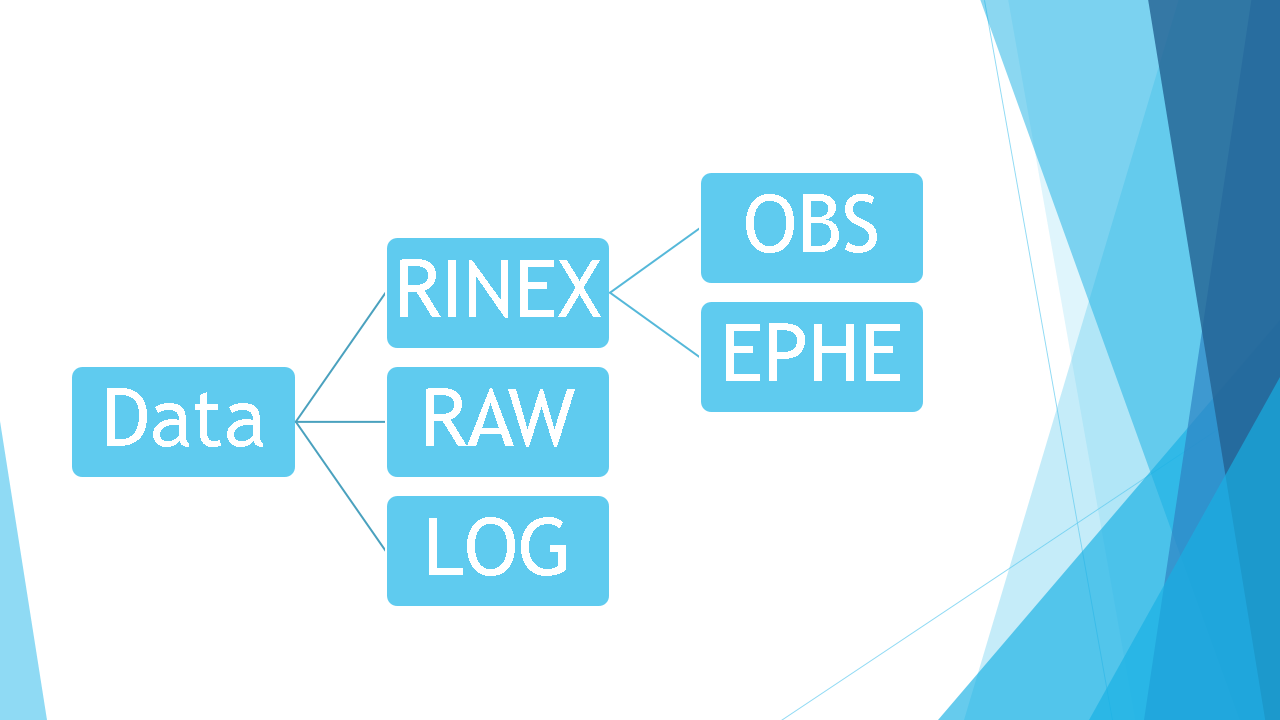
\includegraphics[width=0.95\textwidth]{images/Estructura_de_directorios}
\caption{Estructura de directorios - BKG Ntrip Client}
\label{fig:4.3}
\end{figure}

\item \textbf{Herramienta ETL (\emph{Extraction, Transformation, Load}):} Se desarroll'o un software espec'ifico para cumplir con el prop'osito de extraer, transformar y realizar el cargue de los datos a la base de datos. \\

Esta aplicaci'on tiene el nombre de RINEX ETL y fue programada con el lenguaje Java dada la portabilidad que tiene este lenguaje a los diferentes sistemas operativos que se encuentran actualmente en el mercado.
El principal objetivo de la aplicaci'on es la lectura de los \emph{Observation Files}, extracci'on e inserci'on de los datos objetivo de esta investigaci'on en la base de datos.\\

La aplicaci'on se desarroll'o para que se pueda ejecutar de manera secuencial o serial, y de manera paralela, haciendo uso de los cores de los multi-procesadores.\\

La arquitectura de la aplicaci'on est'a basada en dos capas:

\begin{itemize}
\item \textbf{\emph{Parser}:} Es la capa principal de la aplicaci'on dado que se encarga de la lectura, extracci'on y transformaci'on de los datos obtenidos de los \emph{Observation files}. En esta capa se implementa la interface \emph{Runnable} de Java, la cual permite realizar procesamiento en paralelo a trav'es de \emph{Threads} o hilos.
\item \textbf{\emph{Data Access Object (DAO)}:} Esta capa suministra la interfaz com'un entre la aplicaci'on y la base de datos (componente de almacenamiento), es decir, la que permite la comunicaci'on entre el componente de almacenamiento y la aplicaci'on.
\end{itemize}

\begin{figure}[H]
\centering
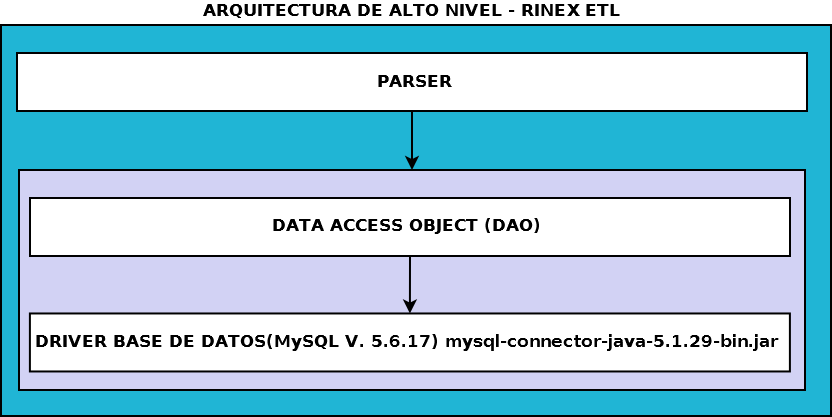
\includegraphics[width=0.95\textwidth]{images/ARQUITECTURA_RINEX_ETL}
\caption{Arquitectura de alto nivel, RINEX ETL}
\label{fig:4.4}
\end{figure}

Entrando un poco m'as en detalles, la aplicaci'on est'a compuesta por sus propios componentes y paquetes, como tambi'en hace uso de unas librer'ias de uso libre(\emph{Freeware}), las cuales hacen parte de los componentes reusables del programa. La aplicaci'on tiene una alta dependencia de estas librer'ias para la comunicaci'on con la base de datos tanto para la forma secuencial como para la paralela, tal como se puede evidenciar en la siguiente figura.

\begin{figure}[H]
\centering
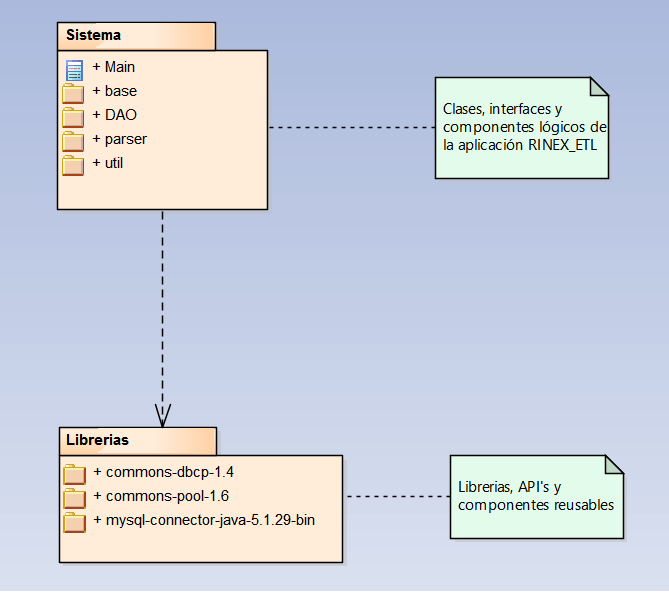
\includegraphics[width=0.95\textwidth]{images/Component_Diagram}
\caption{Diagrama de componentes, RINEX ETL}
\label{fig:4.5}
\end{figure}

Igualmente dentro de las librerias usadas, se tienen unas dependencias, las cuales est'an relacionadas con aquellos componentes para la creaci'on de un \emph{Pool} de conexiones hacia la base de datos. Este \emph{pool} es utilizado para la forma paralela dada la concurrencia que se maneja en este tipo de ejecuci'on. \\

En la figura de abajo se muestran las dependencias internas entre las librer'ias usadas por la aplicaci'on. 

\begin{figure}[H]
\centering
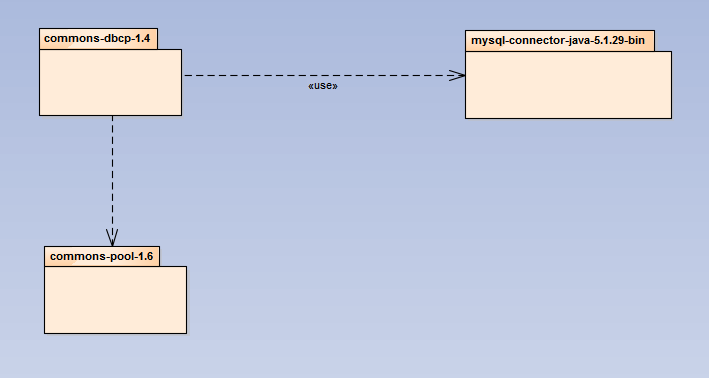
\includegraphics[width=0.95\textwidth]{images/Library_Diagram}
\caption{Diagrama de librerias, RINEX ETL}
\label{fig:4.6}
\end{figure}

Continuando con la descripci'on del programa, se presenta la distribuci'on interna o de paquetes, en la cual se observan las clases que hacen parte de cada uno de los mismos.

\begin{itemize}
\item \textbf{\emph{Default}:} Se encuentra la clase que ejecuta la aplicaci'on y mantiene la configuraci'on especificada para la misma.
\item \textbf{Base:} Se encuentran las clases o estructuras de datos utilizados a lo largo de la aplicaci'on como la metadata y los datos de las observaciones.
\item \textbf{\emph{Data Access Object (DAO)}:} Se encuentran las clases que implementan la inserci'on de los datos extra'idos y la comunicaci'on con el componente de almacenamiento.
\item \textbf{\emph{Parser}:} Es la clase que se encarga de la lectura, extracci'on y transformaci'on de los datos obtenidos de los \emph{Observation files}.
\item \textbf{Util:} Est'an las constantes utilizadas en la mayor parte de la aplicaci'on, como las clases que hacen uso del \emph{driver} de la base de datos para la creaci'on de conexiones hacia esta.
\end{itemize}

\begin{figure}[H]
\centering
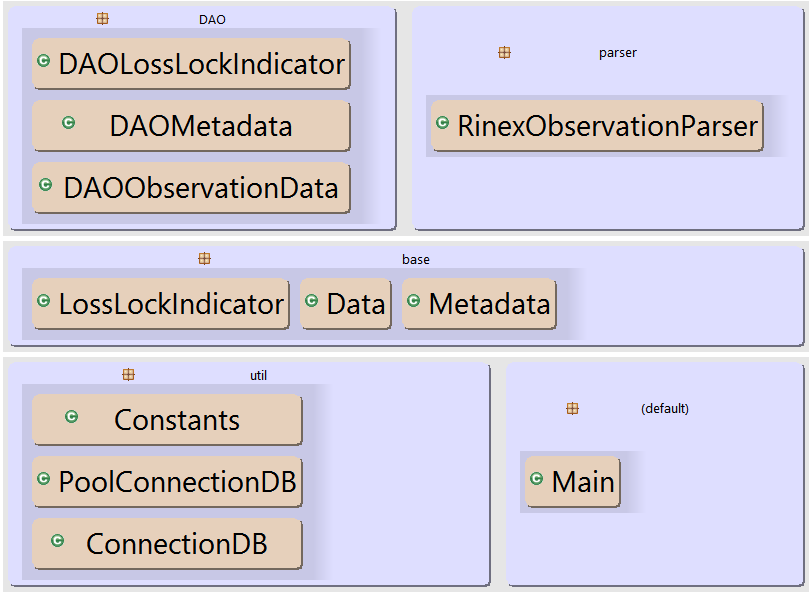
\includegraphics[width=0.95\textwidth]{images/Package_Diagram}
\caption{Diagrama de paquetes, RINEX ETL}
\label{fig:4.7}
\end{figure}

Finalizando con la especificaci'on del software desarrollado y como 'ultima parte de detalle se muestra el diagrama de clases con sus respectivas relaciones entre las mismas, sus atributos y sus m'etodos.

\begin{figure}[H]
\centering
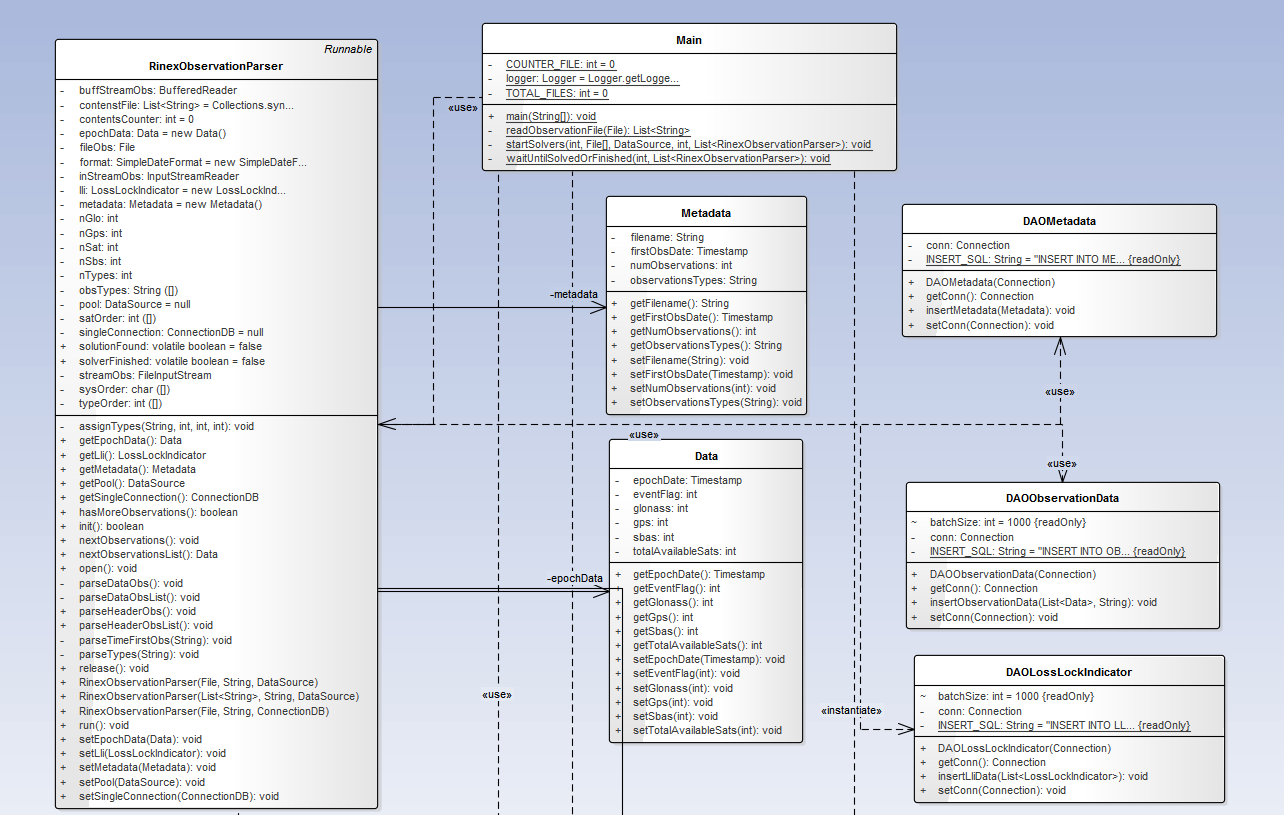
\includegraphics[width=0.95\textwidth]{images/Class_Diagram_1}
\caption{Diagrama de clases, parte 1, RINEX ETL}
\label{fig:4.8}
\end{figure}

\begin{figure}[H]
\centering
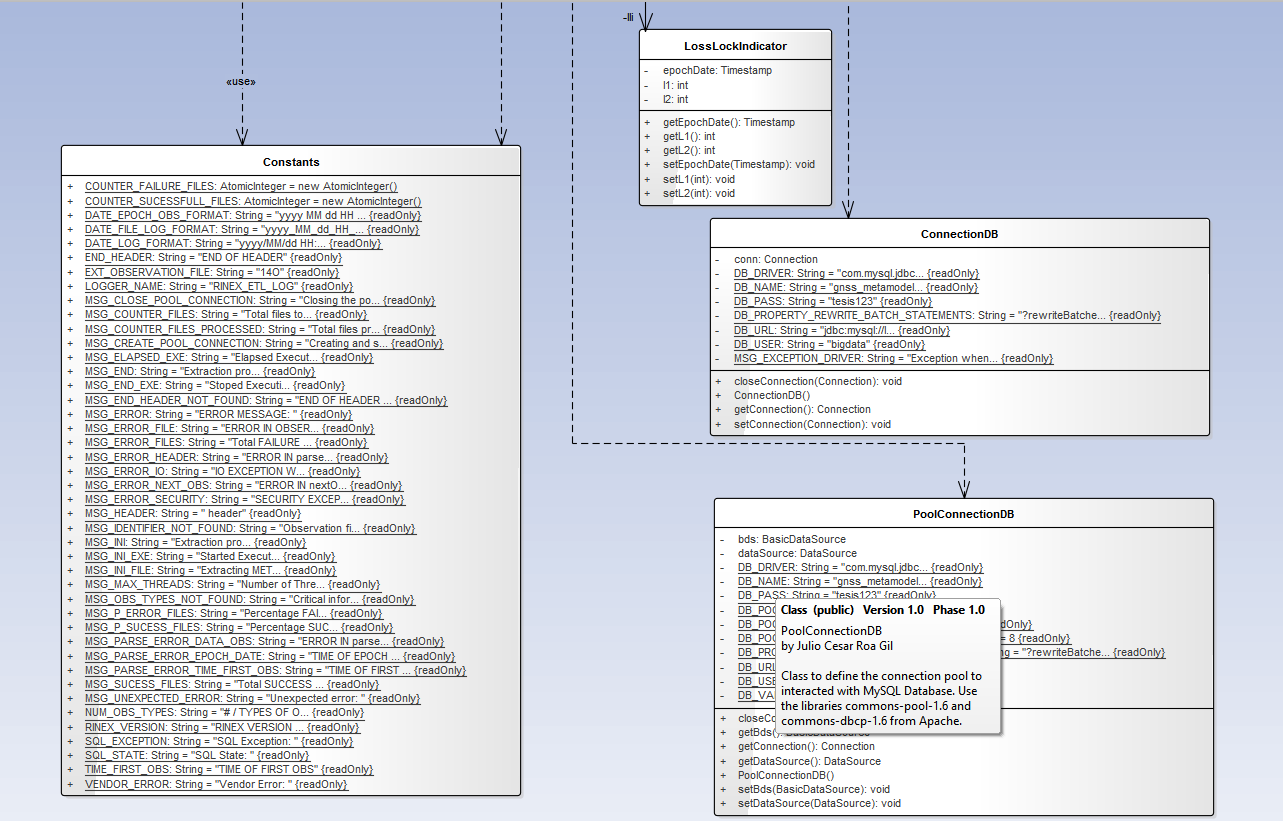
\includegraphics[width=0.95\textwidth]{images/Class_Diagram_2}
\caption{Diagrama de clases, parte 2, RINEX ETL}
\label{fig:4.9}
\end{figure}

Las dos principales clases utilizadas son: \emph{Main y RinexObservationParser}, para la extracci'on y transformaci'on. El \emph{Main} es el punto de partida de la aplicaci'on y es en la cual se configura el directorio de archivos a leer, el modo de operar (secuencial o paralelo), es decir, la especificaci'on del n'umero de hilos, y la ruta para el archivo \emph{log} o bit'acora del programa. El \emph{RinexObservationParser} se encarga de abrir, leer y cerrar los \emph{Observation files}, y a su vez realizar el paso de los datos extra'idos hacia los \emph{Data Access Objects} para su posterior inserci'on en la base de datos. \\

Los \emph{DAO's} por su parte realizan la comunicaci'on con la base de datos y la operaci'on de escritura o inserci'on en la misma. Esta operaci'on fue optimizada a trav'es de las librerias JAVA haciendo los llamados a las funciones de \emph{Bulk Inserts} o \emph{Batch processing} con lo cual se mejora notablemente el rendimiento cuando es necesario introducir grandes cantidades de datos.\\

Las clases \emph{ConnectionDB} y \emph{PoolConnectionDB} que se encargan de implementar como tal la comunicaci'on directa con la base de datos al hacer uso del \emph{Driver mysql-connector-java-5.1.29-bin.jar}. La primera clase implementa una sola conexi'on y se utiliza para la ejecuci'on secuencial, y la  segunda clase implementa un \emph{Pool} de conexiones, o mantiene varias conexiones abiertas para que los diferentes \emph{Threads} las utilicen. Este \emph{pool} de conexiones es configurable para colocar los l'imites de conexiones abiertas, en espera, y en ejecuci'on.

\end{enumerate}

\subsection{Componente de almacenamiento}
\noindent
Aqu'i encontramos la base de datos con el meta-modelo definido para almacenar y extraer la informaci'on de inter'es definida para esta investigaci'on. La base de datos es relacional por lo que nuestro meta-modelo se dise'n'o bajo un diagrama de entidad/relaci'on, el cual se ilustra a continuaci'on.

\begin{figure}[H]
\centering
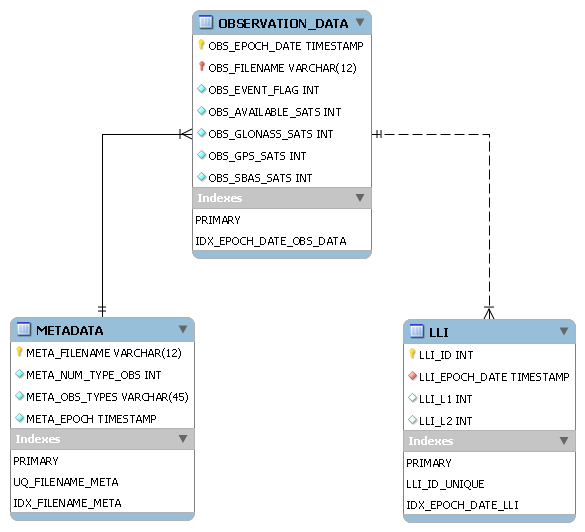
\includegraphics[width=0.95\textwidth]{images/ER}
\caption{Meta-modelo - Diagrama Entidad/Relaci'on}
\label{fig:4.10}
\end{figure}

Como se puede observar existen dos tablas, las cuales representan de cierta manera el \emph{header} y el \emph{body} de los \emph{observations files} en formato RINEX. Estas tablas contienen los campos necesarios para poder relacionar la informaci'on m'as importante y extraer as'i el conocimiento de este conjunto de informaci'on. La tercera tabla es mucho m'as espec'ifica, y almacena los datos referentes al \emph{Loss of Lock Indicator (LLI)} de los tipos de observaciones L1 y L2, su raz'on de ser es la de encontrar los posibles deslizamientos de los ciclos en las \emph{Epoch Dates} con el objetivo de analizar las medidas realizadas por los \emph{GNSS}.

\section{Proceso de descarga}
\noindent
Esta secci'on explica c'omo funciona el proceso de descarga implementado en esta investigaci'on y se hace por medio de un diagrama de flujo para entender el proceso de una manera visual.

\begin{figure}[H]
\centering
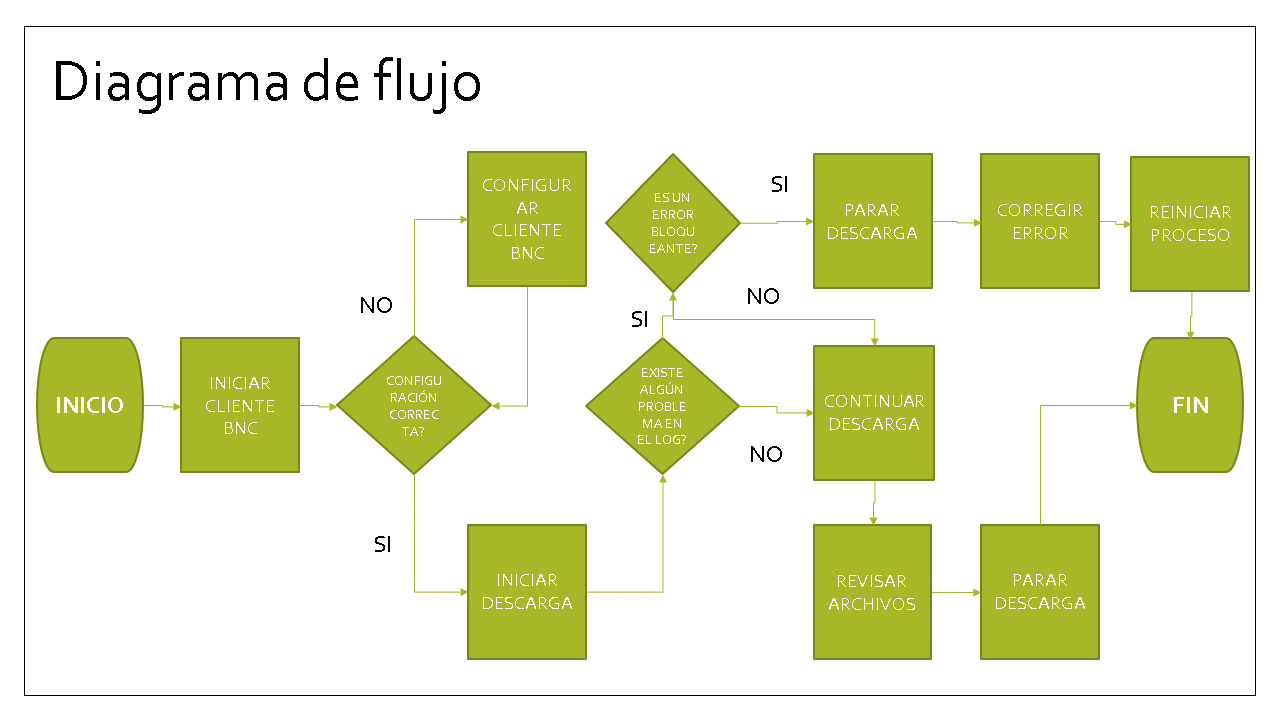
\includegraphics[width=0.95\textwidth]{images/Proceso_de_descarga}
\caption{Diagrama de flujo - Proceso de descarga}
\label{fig:4.11}
\end{figure}

\clearpage